\documentclass[10pt,conference]{IEEEtran}
\IEEEoverridecommandlockouts
% The preceding line is only needed to identify funding in the first footnote. If that is unneeded, please comment it out.
\usepackage{cite}
\usepackage{amsmath,amssymb,amsfonts}
\usepackage{algorithmic}
\usepackage{graphicx}
\usepackage{textcomp}
\usepackage{booktabs}
\usepackage[table,xcdraw]{xcolor}
\usepackage{framed}
\usepackage{xcolor}
\definecolor{mypink3}{cmyk}{0, 0.7808, 0.4429, 0.1412}

\def\BibTeX{{\rm B\kern-.05em{\sc i\kern-.025em b}\kern-.08em
    T\kern-.1667em\lower.7ex\hbox{E}\kern-.125emX}}

\begin{document}

\title{Security vs. Maintainability: Fixing Vulnerabilities Obfuscates your Code%\\
%\thanks{Identify applicable funding agency here. If none, delete this.}
}

\author{
    Anonymou(s) Author(s)
%     \IEEEauthorblockN{1\textsuperscript{st} Given Name Surname}
% \IEEEauthorblockA{\textit{dept. name of organization (of Aff.)} \\
% \textit{name of organization (of Aff.)}\\
% City, Country \\
% email address}
% \and
% \IEEEauthorblockN{2\textsuperscript{nd} Given Name Surname}
% \IEEEauthorblockA{\textit{dept. name of organization (of Aff.)} \\
% \textit{name of organization (of Aff.)}\\
% City, Country \\
% email address}
% \and
% \IEEEauthorblockN{3\textsuperscript{rd} Given Name Surname}
% \IEEEauthorblockA{\textit{dept. name of organization (of Aff.)} \\
% \textit{name of organization (of Aff.)}\\
% City, Country \\
% email address}
}

\maketitle

\begin{abstract}
  Security is a crucial non-functionality requirement for software applications.
  However, building secure software is far from trivial as developers lack both
  the knowledge and tools to effectively address this concern. In this paper, we
  study the impact of changes to improve security on the maintainability of several
  open source applications. Using a dataset containing $607$ security-oriented
  commits, we measure maintainability --- as computed by the Software Improvement
  Group's web-based source code analysis service \emph{Better Code Hub} (BCH) ---
  before and after the security refactoring. Results show that making software
  more secure comes at a cost on maintainability. This is particularly evident
  in refactorings to deal with \textit{Broken Authentication} and \textit{Cross-Site Request Forgery} attacks.
  \textcolor{mypink3}{Furthermore, we have found evidence that security-related changes are more
  likely to be modified in the future than regular code changes.}
\end{abstract}

\begin{IEEEkeywords}
Security, Software Maintenance, Open-Source Software
\end{IEEEkeywords}

\section{Introduction}



The international standard ISO/IEC 25010:2011 breaks down software quality into eight characteristics: maintainability,
functional suitability, performance efficiency, compatibility, usability, reliability, security,
and portability. This paper focuses solely on maintainability.



\section{Motivation and Research Questions}

\textcolor{mypink3}{Ver que exemplos existem na amostra da secbench que vamos utilizar para dar como exemplo de motivacao}

\begin{framed}
\textit{\textbf{RQ1} What is the impact of security refactorings on the maintainability of open-source software?}
\end{framed}

\begin{framed}
\textit{\textbf{RQ2} Which patterns of security refactorings are more likely to affect open-source software maintainability?}
\end{framed}

\begin{framed}
\textit{\textbf{RQ3} }
\end{framed}


\section{Methodology}

In this section, the methodology used to measure the impact of security refactorings on the maintainability of open-source software is presented in depth in the following sections and illustrated in Figure \ref{fig:met}. Aiming to answer the research questions presented in this paper, we use a dataset containing $716$ security refactorings collected from open-source software available on GitHub. $648$ of those refactorings were reported in a previous study conducted in 2017 \cite{Reis:2017:IJSSE}. In parallel, a baseline of regular commits was randomly collected from the list of projects of the main dataset to evaluate what is the impact of regular commits on the maintainability of open-source software. The Software Improvement Group's\footnote{SIG's website is available at https://www.softwareimprovementgroup.com/ (Accessed on January 23, 2019)} web-based source code analysis service Better Code Hub (BCH) \footnote{BCH's website is available at https://bettercodehub.com/ (Accessed on January 23, 2019)} was used to collect the maintainability reports for both security and regular commits.


\begin{figure}[h]
 	\centering 	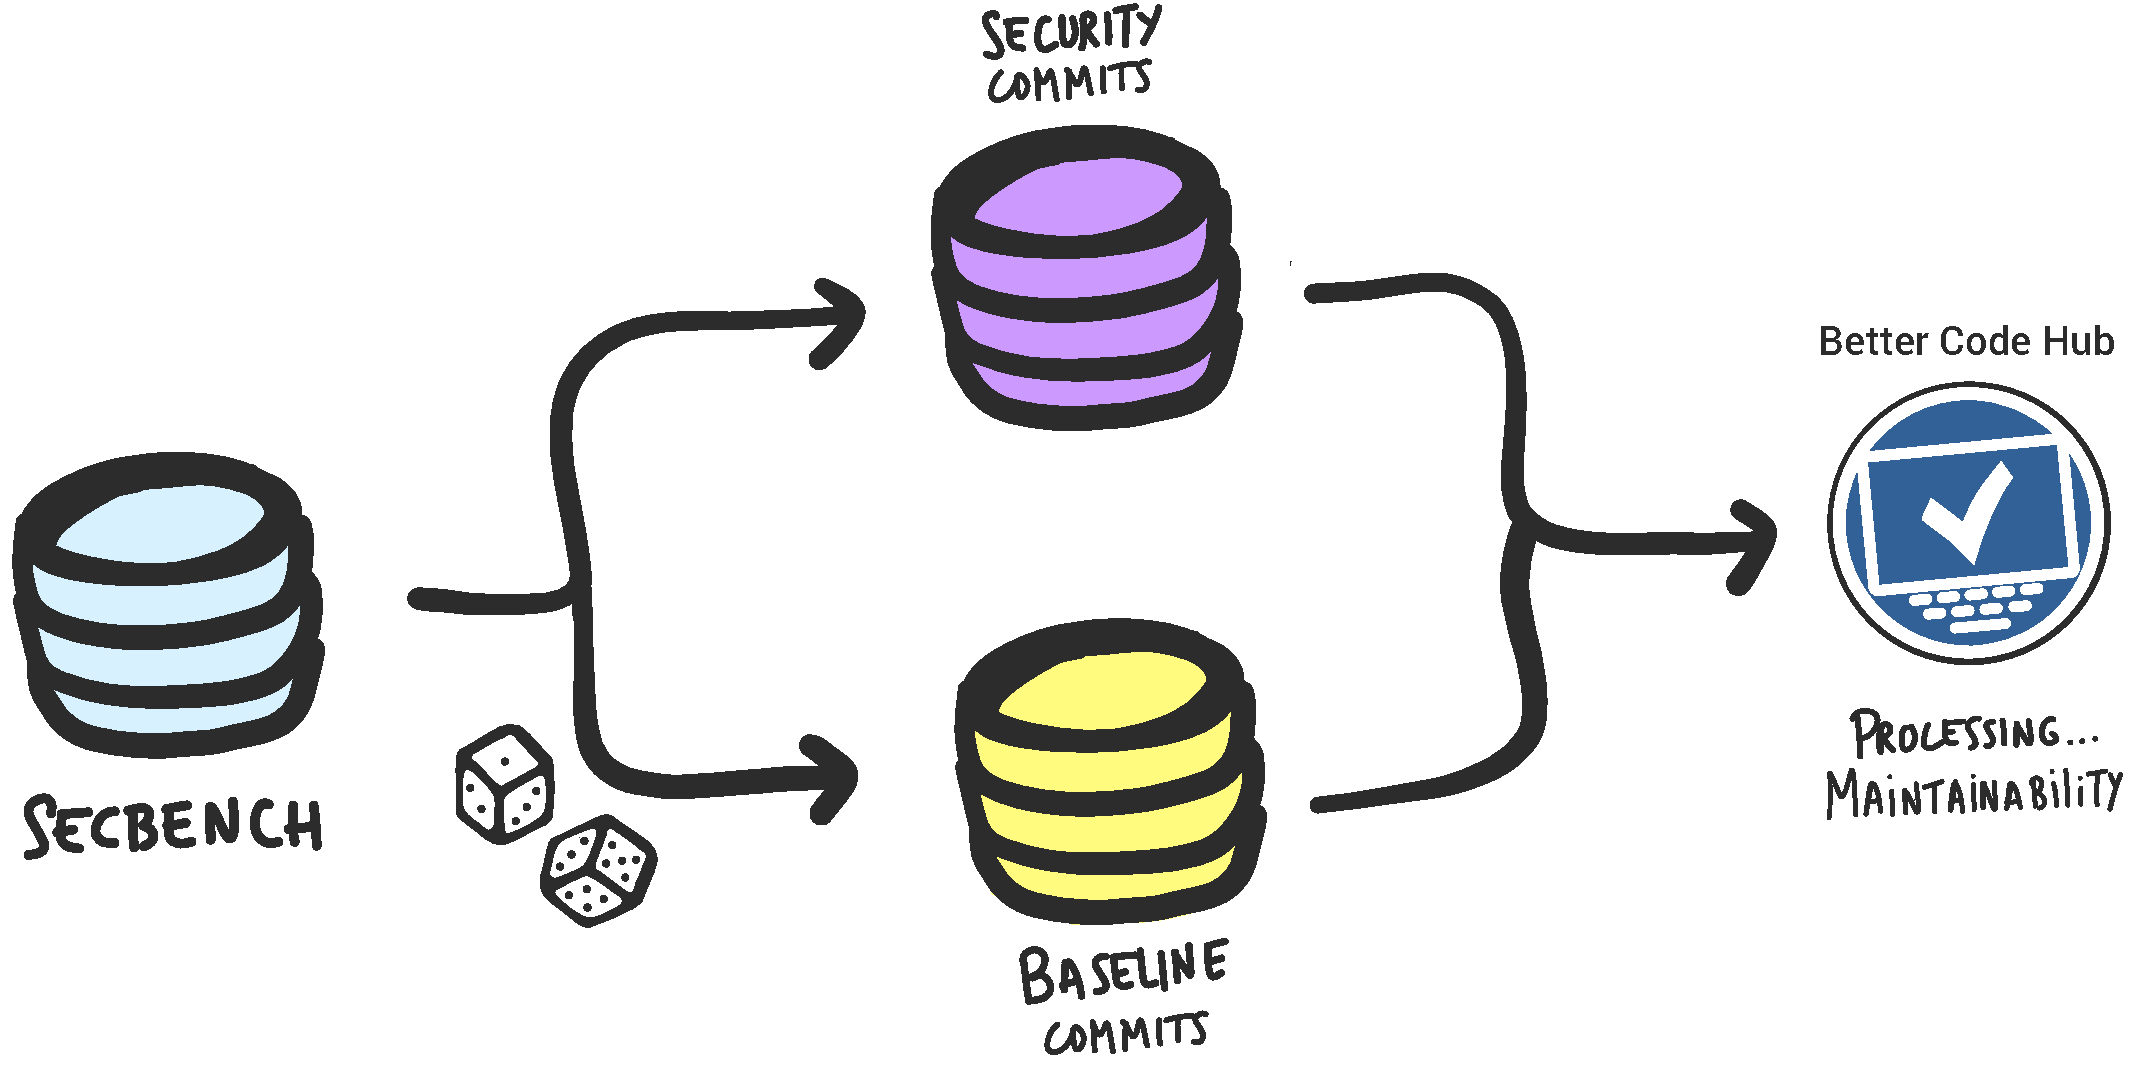
\includegraphics[width=0.5\textwidth]{figures/methodology.pdf}
 	\caption{Study Methodology}
	\label{fig:met}
\end{figure}

\subsection{Dataset}

To evaluate the impact of security refactorings on the maintainability of open-source software, we use a dataset of security flaws which is the outcome of mining more than $248$ GitHub\footnote{Github's website available at https://github.com/ (Accessed on January 23, 2019)} projects. Reis and Abreu (2017) mined open-source software aiming the extraction of real test cases - created by real developers on their daily basis development - to test and assess the performance of static analysis tools since using hand-seeded test cases or mutations could lead to misleading assessments of the capabilities of the tools. The study yielded to a dataset of $648$ test cases for $16$ different patterns. Each test case of the dataset is a triplet of folders: the commit before the refactoring, the commit responsible for the refactoring and the snippets of code that differ from one version to another (usually, called \textit{diff}) - where one can easily identify the code used to fix the security flaw. In this study, we focus on computing the maintainability of the commits before and after the security refactoring to evaluate if the impact was positive, negative or none.

% \begin{table}[h]
% 	\centering
% \caption{Current Dataset Patterns Distribution} \label{tab:patterns}
% \begin{tabular}{@{}ll@{}}
% \toprule
% Pattern & \# Commits\\
% \midrule
% Injection & 89\\
% Broken Authentication and Session Management& 45\\
% Cross-Site Scripting& 142\\
% Broken Access Control& 2\\
% Security Misconfiguration& 9\\
% Sensitive Data Exposure& 24\\
% Insufficient Attack Protection& 18\\
% Cross-Site Request Forgery& 34\\
% Using Components With Known Vulnerabilities& 27\\
% Unprotected APIs& 7\\
% Memory Leak& 91\\
% Overflow& 19\\
% Denial-of-Service& 43\\
% Path Traversal& 19\\
% Resource Leak& 33\\
% SHA-1 Hash Function & 1\\
% Miscellaneous& 101\\\midrule
% Total& 716\\
% \bottomrule
% \end{tabular}
% \end{table}

\begin{figure}[h]
 	\centering
 	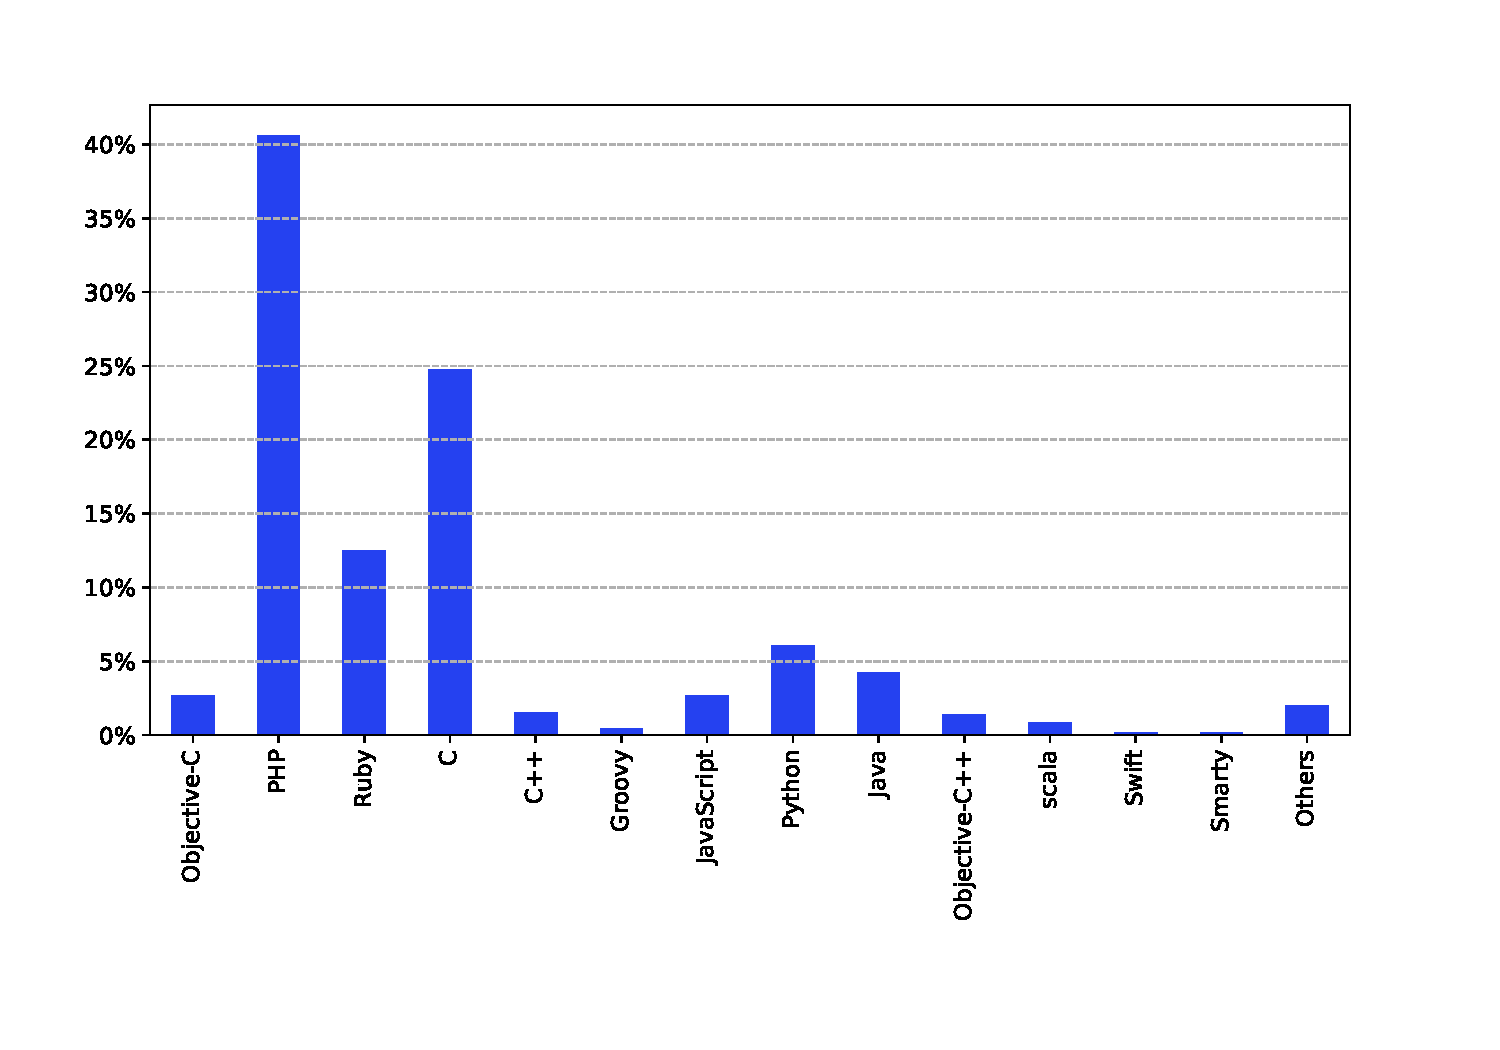
\includegraphics[width=0.5\textwidth]{figures/language_dist.pdf}
 	\caption{Security Refactorings Language Distribution}
	\label{fig:lang}
\end{figure}

\begin{figure}[h]
 	\centering
 	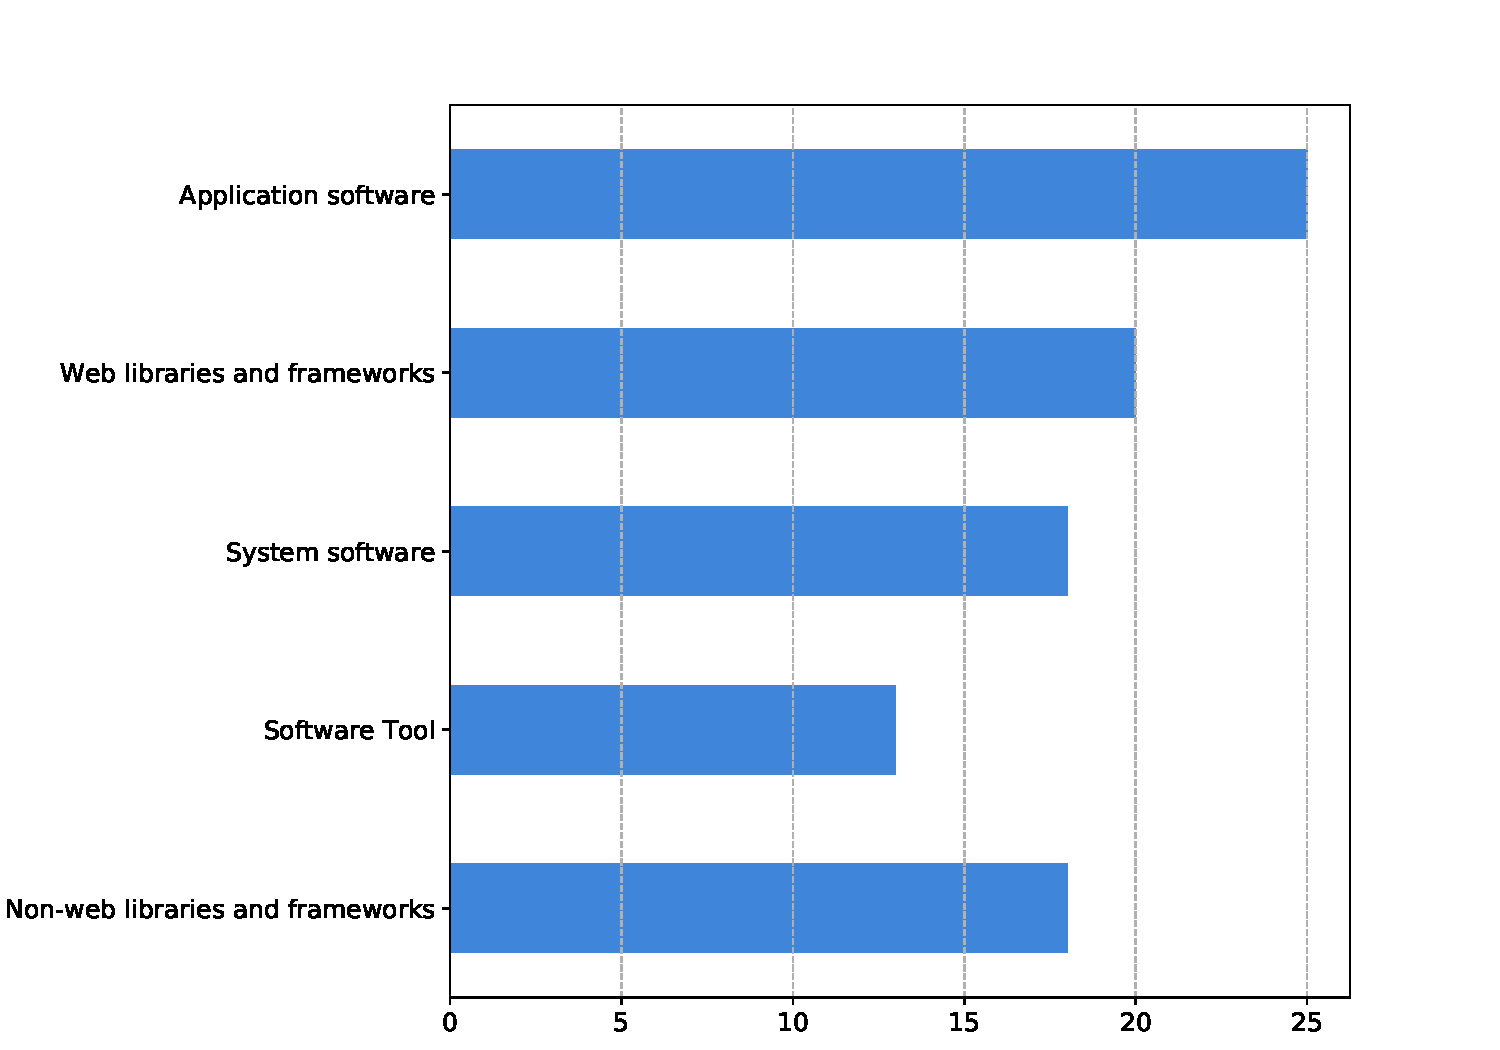
\includegraphics[width=0.5\textwidth]{figures/type_dist.pdf}
 	\caption{Type Distribution}
	\label{fig:type}
\end{figure}

Reis and Abreu ($2017$) dataset commits were manually validated, flagged as security flaws and classified with one of the $16$ following patterns: \textit{Injection}, \textit{Broken Authentication and Session Management}, \textit{Cross-Site Scripting}, \textit{Broken Access Control}, \textit{Security Misconfiguration}, \textit{Sensitive Data Exposure}, \textit{Insufficient Attack Protection}, \textit{Cross-Site Request Forgery}, \textit{Using Components With Known Vulnerabilities}, \textit{Unprotected APIs}, \textit{Memory Leak}, \textit{Overflow}, \textit{Denial-of-Service}, \textit{Path Traversal} and \textit{Miscellaneous}. However, the dataset evolved and now integrates new patterns, such as \textit{Resource Leak} and \textit{SHA-1 Hash Function}. A considerable amount of these patterns are based in the OWASP Top 10 of 2013~\cite{oswap:2013} and OWASP Top 10 of 2017~\cite{oswap:2017}.

In total, the dataset contains 716 security refactorings. These refactorings were computed by the BCH tool to calculate maintainability. However, some of the refactorings are not considered in the final results due to limitations of BCH: lack of language support and project size. The Wilcoxon statistical test - described more in-depth in subsection \ref{sec:statsval} - is performed to evaluate the significance of our results. Each type of security flaw is tested, Figure \ref{fig:pat}. One of the main requirements of this test is that the input sample needs to comprise more than 20 commits. Thus, the patterns not complying with this requirement were reallocated to the \textit{Miscellaneous} pattern. In the end, we highlight the following patterns:

\begin{itemize}
	\item \textbf{Using Components with Known Vulnerabilities.} The majority of software produced today integrates several components, such as libraries and frameworks, which may affect the software if developers use vulnerable versions - usually known and disclosed somewhere on the Internet. \textit{Based on the OWASP Top 10 of 2017.}
	\item \textbf{Broken Authentication \& Session Management.} Uncorrectly implemented functionalities related to authentication and session management, allowing crackers to gain access to session tokens, passwords, keys and other sensitive data \textit{- Based on the OWASP Top 10 of 2013.}
	\item \textbf{Cross-Site Request Forgery.} Poor session tokens generation and management usually allow crackers to send forged HTTP requests including authentication information from the victim to vulnerable web application \textit{- Based on the OWASP Top 10 of 2013.}
	\item \textbf{Denial-of-Service} Security flaws that can allow a cracker to flood or crashing services. This attacks usually occur when the system receives much traffic causing it to slow down and eventually stop. For example, flaws allowing crackers to trigger memory allocations corresponding to large length values (CVE-2014-3506)\footnote{CVE-2014-3506 details available at https://nvd.nist.gov/vuln/detail/CVE-2014-3506 (Accessed on January 25, 2019)}. 
	\item \textbf{Miscellaneous} This pattern comprises several others categories of security refactorings (e.g., \textit{path traversal and buffer overflow}). It contains several other security refactorings that do not have their own pattern yet. The patterns not satisfying the size requirement of more than 20 refactorings are contemplated here.	
	\item \textbf{Cross-Site Scripting.} Lack of proper validation or escaping allow crackers to submit untrusted data to web browsers through malicious scripts that can hijack the user sessions or redirect the user to malicious sites \textit{- Based on the OWASP Top 10 of 2017.}
	\item \textbf{Injection.} When developers do not keep untrusted data separate from commands and queries. If a cracker sends a string that exploits the syntax of the interpreter, then an injection attack is possible (e.g., SQL and LDAP injection)\textit{- Based on the OWASP Top 10 of 2017.}
	\item \textbf{Memory Leak.} Memory management issue found more frequently in programming languages that do not manage memory automatically (e.g., C/C++ and Objective-C), i.e., where instead developers are responsible for handling it. One of the main causes of DoS attacks.
\end{itemize}

The dataset contemplates security flaws for more than 13 different languages being PHP the most prevalent one, Figure \ref{fig:lang}. This may be due to the abundance of web software (e.g., Library, Frameworks, Platform, Server), Figure \ref{fig:type}. 

\begin{table*}[h]
	\centering
	\caption{Descriptive statistics of the dataset projects}
\begin{tabular}{@{}lllllllllll@{}}
\toprule
      & forks   & stars   & watchers & contributors & commits  & branches & releases & size      & issues & pull requests  \\ \midrule
mean  & 1763.52 & 5448.74 & 401.37   & 153.33       & 14834.17 & 45.17    & 129.45   & 122973.24 & 3768.97   & 1941.61 \\
std   & 2434.03 & 6215.09 & 486.60   & 123.68       & 22234.46 & 150.15   & 189.93   & 209732.51 & 5933.16   & 3603.31 \\
min   & 1       & 3       & 1        & 0            & 103      & 1        & 0        & 108       & 0         & 0       \\
25\%  & 391.50  & 1581    & 117.25   & 49           & 1440.50  & 4        & 19       & 8466.75   & 313.75    & 143.25  \\
median  & 838.50  & 2836.50 & 248      & 99           & 5504.50  & 9        & 59       & 37372.50  & 1792.50   & 650     \\
75\%  & 2155    & 6828.50 & 459.50   & 261          & 18579.25 & 20       & 142.75   & 117699.50 & 4087.75   & 1907.25 \\
max   & 16366   & 31841   & 3446     & 413          & 114378   & 1227     & 1114     & 995790    & 33970     & 19329   \\
Total & 165771  & 512182  & 37729    & 14413        & 1394412  & 4246     & 12168    & 11559485  & 354283    & 182511  \\ \bottomrule
\end{tabular}
\label{tab:dataset}
\end{table*}

Table \ref{tab:dataset} presents the final dataset projects statistics. Refactorings from 94 projects were evaluated by BCH. According to the statistics, the projects of this dataset are \textcolor{mypink3}{popular and the developers are active}. 

\subsection{Security vs. Baseline Commits}
%
Although we want to assess the maintainability of security-related commits,
\textcolor{mypink3}{there is no evidence in previous work on the impact of \textit{regular} commits
in the maintainability of projects}. Thus, we analyze the maintainability of
regular commits and use them as a baseline.

The baseline dataset uses the security commits dataset as input. For each
security commit, one random commit is selected from the list of all commits of
the belonging project. We originate the regular commits from the security
commits to ensure that differences in maintainability are not consequence of
characteristics of different projects.
%
\subsection{Maintainability Analysis}

BCH is used to collect the maintanability reports of the commits of each project. The tool
evaluation is based on a model of 10 different guidelines \cite{Visser:2016:OREILLY}:

\begin{itemize}
	\item \textbf{Write short units of code.} Long units are hard to test, reuse, and understand.
	\item \textbf{Write simple units of code.} Keeping the number of branch points low makes units easier to modify and test.
	\item \textbf{Write code once.} When code is duplicated, bugs need to be fixed in multiple places, which is inefficient and
prone to errors.
	\item \textbf{Keep unit interfaces small.} Keeping the number of parameters low makes units easier to understand and reuse.
	\item \textbf{Separate concerns in modules.} Changes in a loosely
coupled codebase are much easier to oversee and execute
than changes in a tightly coupled codebase.
	\item \textbf{Couple architecture components loosely.} Independent
components ease isolated maintenance.
	\item \textbf{Keep architecture components balanced.} Balanced
components ease locating code and foster isolation,
improving maintenance activities.
	\item \textbf{Keep your codebase small.} Small systems are easier to
search through, analyze, and understand code.
	\item \textbf{Automate tests.} Automated testing makes development
predictable and less risky.
	\item \textbf{Write clean code.} Code without code smells is less likely to bring maintainability issues.
\end{itemize}

For each guideline, BCH evaluates the compliance against a particular guideline by setting boundaries for the percentage of code allowed to fall in each of the four risk severity categories (low risk, medium risk, high risk, and very high risk). If the thresholds are not violated, the project is considered to be compliant with the guideline. According to BCH, the guideline thresholds are calibrated yearly based on a representative benchmark of closed and open-source software systems. Being compliant with a guideline means that the project under analysis is at least better than 65\% of the software systems in BCH’s benchmark.

The BCH report of the $<INSERT\_EXEMPLO>$ for a non-compliant guideline can be seen in Fig. [X]. This was extracted from the report of the app $<INSERT\_EXEMPLO>$, used in the motivating example of Section II [MAYBE?]. The green bar represents the percentage of compliant lines of code. These lines of code are considered to be compliant with ISO 25010 standard for maintainability [21]. The yellow, orange and red bars represent non-compliant lines of code with medium, high, and very high severity levels, respectively. Along the bars, there are also marks that refer to the compliance thresholds for each severity level. The report is equivalent to the information reported in Table II: a set of thresholds, number of lines of code (LOC), and percentage of the project for each severity level. Nonetheless, thresholds provided by BCH do not sum to 100\%: non-compliant levels are provided in a cumulative way (e.g., the threshold for the medium level includes high and very high levels); the compliant-level threshold is the complement of the medium-level threshold.

Since we want to analyze maintainability regression, we
use BCH to compute maintainability in two different versions of the Android app: a) the version of the project before the security commit ($v_{E-1}$) and b) the version immediately after the security commit ($v_E$). This is illustrated in Fig. [X].
Although BCH provides a detailed report of the maintainability of the project, it does not compute a final score that we can use to compare maintainability amongst different projects. Thus, based in previous work CITE?, we designed an equation to capture the distance between the current state of the project and the standard thresholds. We have adjusted the equation to meet the following requirements:

\begin{itemize}
	\item \textbf{The maintainability difference between two versions of the same project is not affected by its size.} In this work, we want to evaluate the identical security patterns occurring in different projects. Thus, the metric cannot use normalization based on its size – we convert percentage data to the respective number of lines of code.
	\item \textbf{Distance to the thresholds in high severity levels is more penalized than in low severity levels.} We use weights based on the severity level to count lines of code that violate maintainability guidelines.
\end{itemize}

We compute the mean average of the maintainability score $M(v)$ for all the selected guidelines, as follows:

\begin{equation}
    M(v) = \sum_{g \in G}^{} M_{g}(v)
\end{equation}

where $G$ is the group of selected maintainability guidelines from BCH (e.g., Write short units of code, etc.) and $v$ is the
version of the software under evaluation. The maintenance $M$ based on the guideline $g$ for a given version of a project is computed with the following equation:

\begin{equation}
    M_{g} = \frac{1}{|L|} \sum_{l \in L}^{} C(l) , L = \{medium, high, veryHigh\}
\end{equation}

where $C$ is the compliance with the maintainability guideline for the given severity level (medium, high, and very high) and
$L$ is the group of severity levels of maintainability infractions. The compliance $C$ for a given severity level $l$ is derived by:

\begin{equation}\label{eq:3}
    C(l) = LOC_{compliant}(l) - w(l) * LOC_{\neg compliant}(l)
\end{equation}

where $LOC_{compliant}(l)$ are the lines of code that comply with the guideline at the given severity level $l$, $LOC_{\neg compliant}(l)$ are the lines of code that do not comply with the guideline at the given
severity level $l$ and $w(l)$ is the weight factor to boost the impact of
non-compliant lines in comparison to compliant lines. Finally, the term $w(l)$ is calculated as follows:

\begin{equation}
    w(l) = \frac{1 - T(l)}{T(l)}
\end{equation}

where $T(l)$ is the threshold in percentage of the lines of code that are accepted to be non-compliant with the guideline for the severity level $l$. This is a standard value defined by BCH. In other words, the factor $w$ is used in Eq. \ref{eq:3} to highlight the lines of code that are not complying with the guideline. For instance, the threshold for the severity level veryHigh is defined in Table II as T(veryHigh) = 6.9\%, which derives to a weight of w(veryHigh) = 13.5. This means that, in this example, one non-compliant guideline is decreasing maintainability score by 13.5 points while a compliant guideline is increasing by 1.0 point. In addition, a version that is perfectly aligned with the standard thresholds has a maintainability score of zero. Then, we compute the difference of maintainability between the security commit ($v_E$) and its parent commit ($v_{E-1}$), as illustrated in Fig. [X].

\subsection{Statistical Validation}\label{sec:statsval}

To validate the maintainability differences in different groups of commits (e.g., baseline and security commits) we use the Paired Wilcoxon signed-rank test with the significance level $\alpha = 0.05$. In other words, we test the null hypothesis that the maintainability difference between pairs of versions $v_{E-1}$, $v_E$ (i.e., before and after an security-commit) follows a symmetric distribution around 0. To understand the effect-size, as advocated by the Common-language effect sizes [X], we compute the mean difference, the median of the difference, and the percentage of cases that reduce maintainability.

\textcolor{mypink3}{@todo: Discuss pratt improvement and accuracy}

\section{Results}


\begin{figure}[h]
 	\centering
 	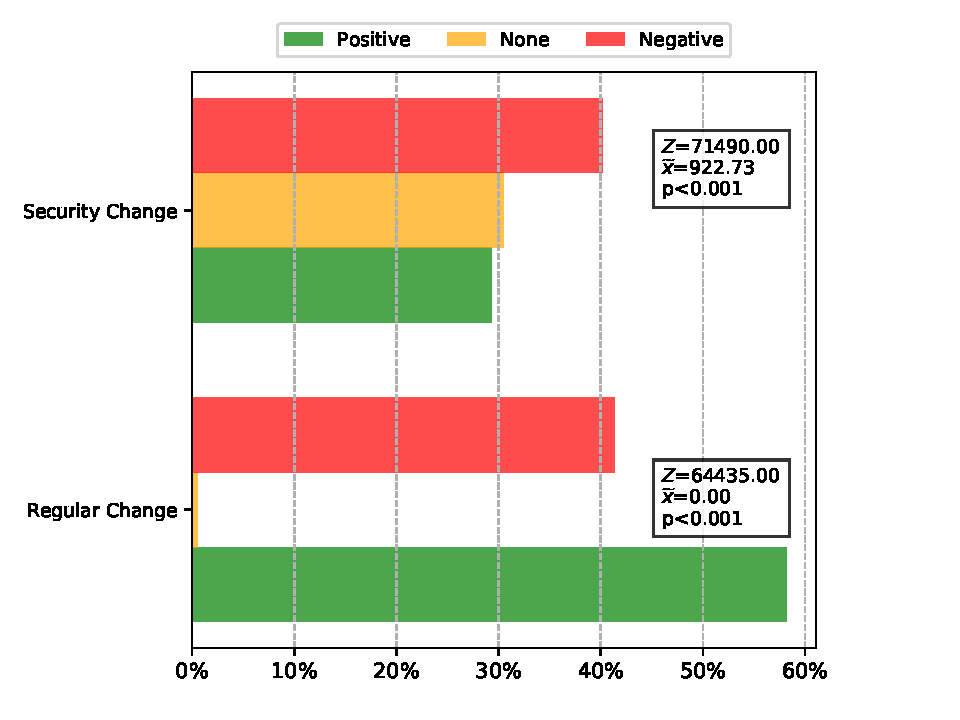
\includegraphics[width=0.45\textwidth]{figures/maintainability.pdf}
 	\caption{Maintainability difference for security and baseline refactorings}
	\label{fig:secvsreg}
\end{figure}

\begin{figure}[h]
 	\centering
 	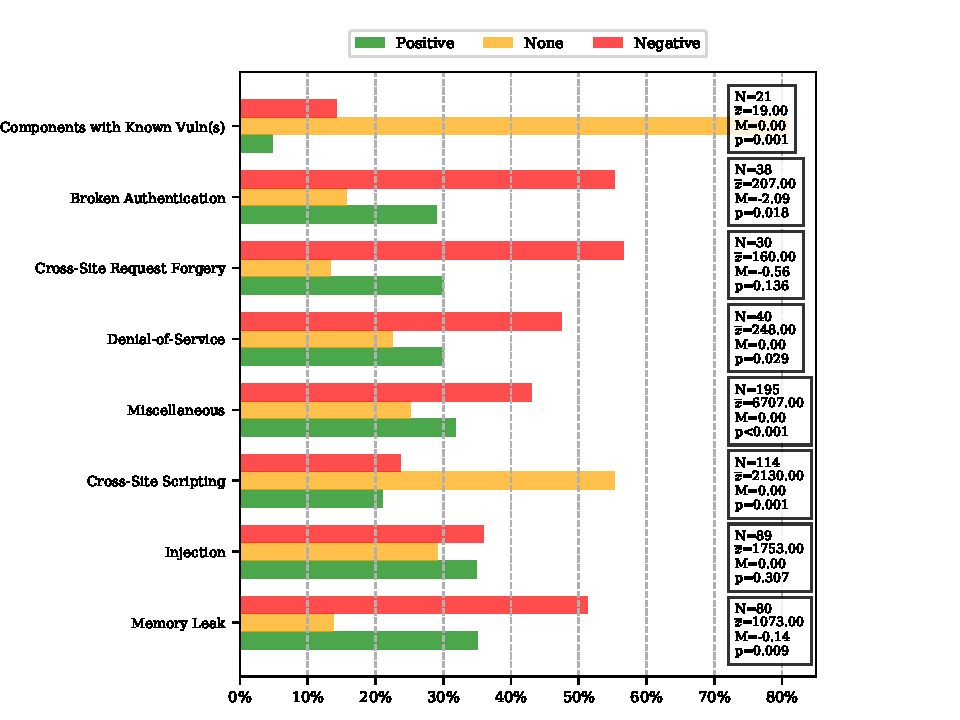
\includegraphics[width=0.55\textwidth]{figures/category.pdf}
 	\caption{Maintainability difference by type after security refactorings}
	\label{fig:pat}
\end{figure}



\begin{framed}
\textit{\textbf{RQ1} What is the impact of security refactorings on the maintainability of open-source software?}
\end{framed}

\begin{framed}
\textit{\textbf{RQ2} Which patterns of security refactorings are more likely to affect open-source software maintainability?}
\end{framed}

\section{Discussion}


\section{Threats to Validity}

\section{Related Work}


\section{Conclusion and Future Work}



\section*{Acknowledgment}

Better Code Hub?

{
 \bibliographystyle{IEEEtran}
  \bibliography{icpc19}
}

\end{document}
